% The programs' execution complexity affects our daily life from many perspectives.
% For example,
% from the privacy and security perspective,
% how much secret information is leaked by a program depends on the number of times a certain operation that leaks the data,
% is executed~\cite{Malacaria07};
% the amount of perturbation in the output data values resulting
% from a small perturbation or uncertainty in the input,
% values depend on the number of times additive error propagation operators are applied; etc.
% Estimating such quantitative properties requires us to know
% how many times is a given control location inside the program that performs certain operations executed?
% % \\
% From the performance perspective, it is important to give a precise estimation
% on the program's resource cost bound w.r.t. the program's inputs.
% For example, in memory-constrained environments such as embedded systems,
% it is important to bound the amount of memory required to run certain applications.
% In real-time systems, it is important to bound the worst-case execution time of the program.
% Applications running on low-power devices or low-bandwidth environments must use up little power or bandwidth respectively. 
% With the advent of cloud computing, where users would be charged per program execution,
% predicting resource usage characteristics would be a crucial component of accurate bid placement by cloud providers. 
% One of the challenges in bounding this cost precisely is that resource consumption is location-sensitive.
% In other words, 
% Different location has different resource cost as well as different execution times. 
% To give accurate estimation results on these execution properties,
% the fundamental questions that need to be addressed 
% is estimating the bound on the execution times
% a given control location inside the program that consumes these resources.
% For these reasons, this paper focuses on analyzing the bound on the execution times of a program's given control location.
% This bound is referred to as the reachability-bound in the program analysis area,
% which is firstly proposed by the paper~\cite{GulwaniZ10}.
% In this paper, finding a symbolic worst-case bound on this quantitative reachability property
% in terms of the inputs to that procedure
% is referred to as the \emph{reachability-bound problem}.

A tight reachability-bound can help to improve the analysis result on other program features.
For example from the privacy and security perspective,
how much secret information is leaked by a program depends on the number of times a certain operation that leaks the data,
is executed~\cite{Malacaria07};
from the efficiency perspective, when different program location consumes different resources, it is important to give a precise estimation on reachability-bound on each location.
While most of existing works all have their limitations in inferring the \emph{reachability-bound} for each location and doesn't compute a good solution to this  problem.
The paper~\cite{GulwaniZ10} that introduces this concept
gives a two-step solution by combining the abstract interpretation and proof-rules-based techniques but not solve this problem in a path-sensitive manner.
% However, their solution
% does not solve this problem in a path-sensitive manner.
It over-approximates the reachability-bounds on different paths inside a while loop.
% \\
Works in program complexity analysis~\cite{GustafssonEL05,HumenbergerJK18} or worst-case resource cost analysis
~\cite{BrockschmidtEFFG16,AlbertAGP08,AliasDFG10,Flores-MontoyaH14} focus only on estimating 
the overall complexity.
% There are also many works in analyzing the program complexity~\cite{GustafssonEL05,HumenbergerJK18},
% or estimating the upper bound on a program's worst-case resource cost
% ~\cite{BrockschmidtEFFG16,AlbertAGP08,AliasDFG10,Flores-MontoyaH14}.
% But their analysis
% focus only on estimating 
% the overall complexity 
% by inferring the bounds on the loop iteration numbers,
% or the worst-case running time and resource cost of the program's entire execution.
None of them computes the reachability-bound on a given program control location directly or path-sensitively.
% \todo{Combine the next two limitations with the general limitations above}
To solve 
the reachability-bounds problem efficiently and path-sensitively, 
we introduce a novel path-sensitive reachability-bound analysis algorithm that combines amortized complexity analysis and loop summarization based loop path refinement techniques. 
\todo{shorten and move to related work, rewrite into how I'm using the two lines of works}
\begin{itemize}
  \item The first one lines up the \emph{amortized complexity analysis} originated from Tarjan's influential paper~\cite{PotechinP17} combined with ranking function~\cite{BradleyMS05} or counter increment and developed in~\cite{ZulegerGSV11,SinnZV14,SinnZV17,LuCT21,AliasDFG10}.
  They do well in nested loops by alternating the loop bound computation with the ranking or counter estimation. This alternation is efficient without recursively unrolling the nested loops when composing the bound of different paths.
  % \\
 But estimating the counter or ranking function invariant ignores the interleaving between multiple paths in the same loop.
Most of them over-approximate the loop bound when the path interleaving affects the loop execution.
  \item 
  Another line of loop bound analysis through loop summarization and path refinement seek for precise loop path representation~\cite{ManoliosV06,BalakrishnanSIG09,SharmaDDA11,Flores-MontoyaH14,HumenbergerJK18,CyphertBKR19}, and compute loop bound over accurate loop summarization~\cite{GulwaniJK09,ZulegerGSV11}.
  They do well in summarizing the loop path and computing the interleaving between paths, and computing a precise bound.
  \\
  The limitation occurs when composing the bound between nested loops. Recursively unrolling the nested loops and computing the interleaving between unrolled paths are heavy and non-terminating.
\end{itemize}
% \todo{more details}
The effective combination complements the limitations in both lines. 
% Based on an abstract transition graph through program abstraction presented in Section~\ref{sec:abs_cfg},
We perform both the path refinement and the ranking estimation over an abstract transition graph through program abstraction presented in Section~\ref{sec:abs_cfg}.
Then we utilize the effectiveness of the \emph{amortized complexity analysis} by computing the ranking function $\locbound(\absevent, c)$ for each transition edge $\absevent$, and estimating the bound on each ranking function.
% , $\varinvar(\locbound(\absevent, c), c)$ and transition edge, $\absclr(\absevent, c)$ alternatively and path-insensitively.
In the meantime, our algorithm is benefited from the accuracy of the path refinement techniques through a light-weight path refinement algorithm adapted from~\cite{GulwaniJK09} presented in Section~\ref{alg:alg-refine_rewrite}.

Build over this combination, we introduce two extra novel quantities,
the \emph{path reachability-bound} and \emph{loop reachability-bound}.
The first one bounds the evaluation times of each loop free and interleaving free path in a refined program, and the second one bounds the iterations of an outer loop w.r.t. the innermost loop such that in these iterations of outer loop, the innermost loop is ``entered''. 
Through estimating the two quantities accurately over the combination, we compute the \emph{reachability-bound} for each program point path-sensitively.
% This combination complements the limitations in both lines.
% % , and computes 
% a \emph{reachability-bound} for every program point $l$ in a program $c$ in a path sensitive manner.
%  as the follows.
% shown in Figure~\ref{fig:psRB-architecture}.
% Based on an abstract transition graph through program abstraction presented in Section~\ref{sec:abs_cfg},
% we perform both the path refinement and the ranking estimation over this graph.
% We utilize the effectiveness of the \emph{amortized complexity analysis} by computing the ranking function $\locbound(\absevent, c)$ for each transition edge $\absevent$, and then estimating the bound on each ranking function, $\varinvar(\locbound(\absevent, c), c)$ and transition edge, $\absclr(\absevent, c)$ alternatively and path-insensitively.
% In the meantime, we also take advantage from the accuracy of the path refinement techniques through a light-weight path refinement algorithm adapted from~\cite{GulwaniJK09} presented in Section~\ref{alg:alg-refine_rewrite}.
% Built on this, we compute the bounds over two novel quantities, the \emph{path reachability-bound} and \emph{loop reachability-bound}. These two bounds effectively combines the strength of the two different bound computation methods above.
% The first key novelty -- the \emph{path reachability-bound} $\inoutB(\rprog, \tpath)$ for a loop free path $\tpath$ within a loop program $\rprog$ bounds the evaluation times of each loop free path instead of the entire multipath loop.
% The second key idea combining two lines of works above is the \emph{loop reachability-bound}, $\lpchB(L:\rprog, \tpath)$.
% For each transition path $\tpath$ w.r.t each of the loops $L:\rprog$ in which $\tpath$ is nested,
% $\lpchB(L:\rprog, \tpath)$ bounds the iterations for
% the outside loop, $L:\rprog$ w.r.t. the innermost loop where $\tpath$ is enclosed,
% such that during these iterations of $L:\rprog$, the innermost loop is ``entered''. 
% Then by multiplication and summing over these two bounds where each program control point shows up, we compute each point's the \emph{reachability-bound} path-sensitively.
% \begin{figure}
% \centering
% 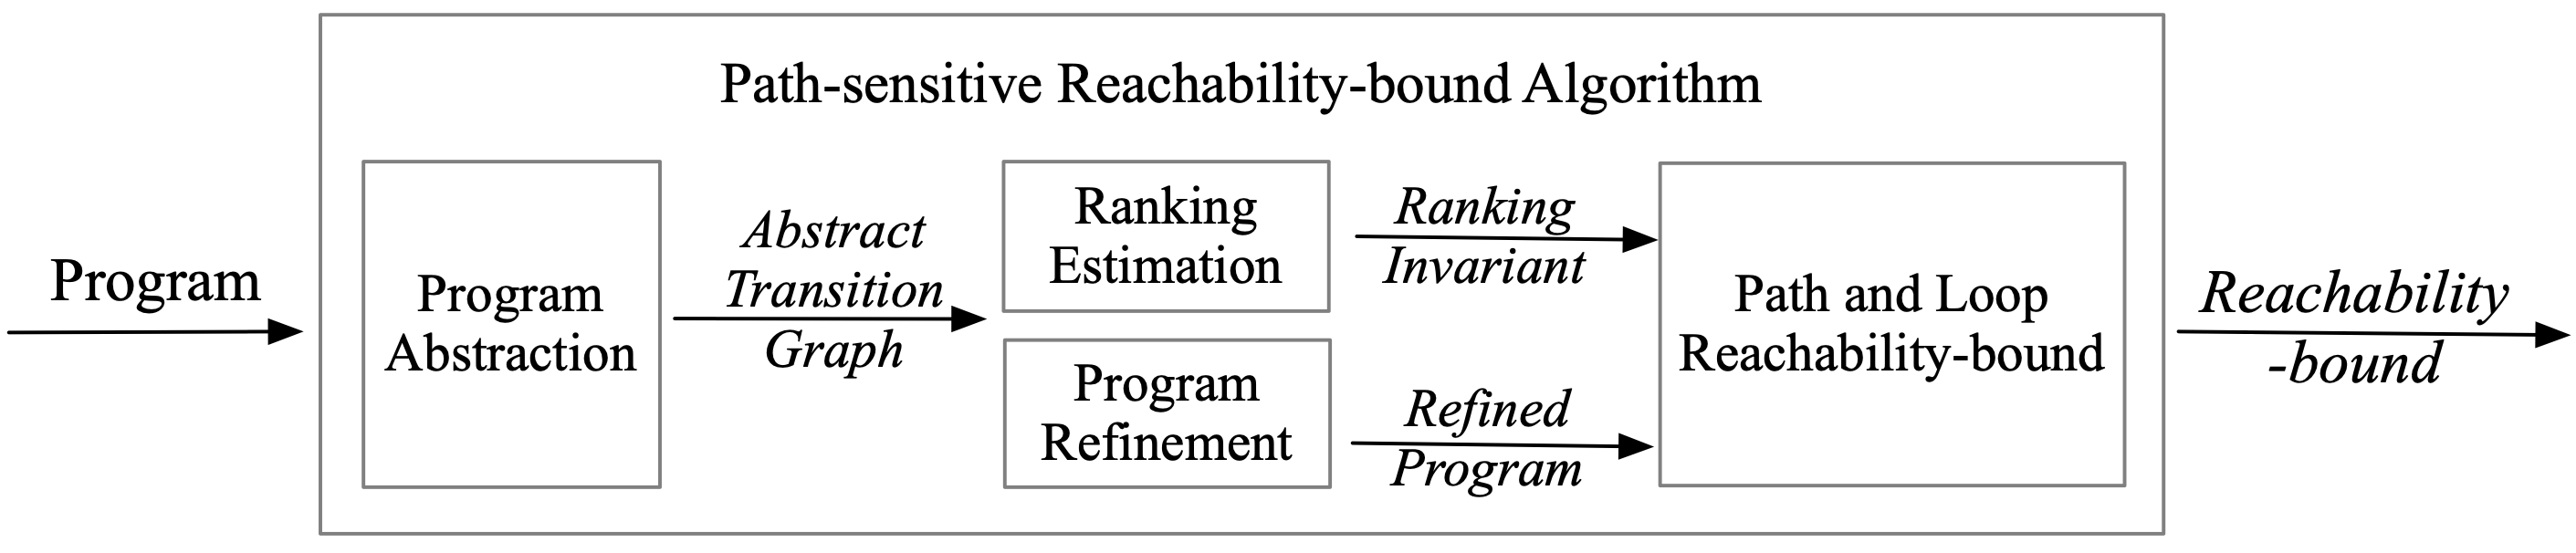
\includegraphics[width=1.0\columnwidth]{psRB-architecture.png}
% \caption{Architecture of the path-sensitive reachability-bound algorithm.}
% \label{fig:psRB-architecture}
% \end{figure}
The main contributions of this work are
\begin{itemize}
  \item 
1. A path-sensitive reachability-bound computation algorithm.
This algorithm can compute the evaluation times of each program point accurately and path-sensitively.
 \item 
2. The combination of the \emph{amortized loop bound analysis} through ranking function estimation and the path refinement based approach in our algorithm.
\item 
3. Two novel quantities, the \emph{path reachability-bound} and \emph{loop reachability-bound} and the corresponding estimating algorithms.
\item 
4. A prototype implementation of this algorithm and an evaluation over four different benchmarks.
  The evaluation results show that we can compute tight bound on the evaluation times of each program point in a program. For program with multi-path loop, we compute different bounds for the points on different paths.
\end{itemize}